\documentclass[10pt]{beamer}

\usetheme{metropolis}
\useoutertheme{metropolis}
\useinnertheme{metropolis}
\usefonttheme{metropolis}
%\usecolortheme{seahorse}   % or your preferred color theme
\usepackage{appendixnumberbeamer}
\usepackage{graphicx}
\usepackage{multirow}
\usepackage{booktabs}
\usepackage[scale=2]{ccicons}
\usepackage{xspace}
\usepackage[justification=centering]{caption}
\usepackage{braket}
\usepackage{amsmath}

\usepackage[version=3]{mhchem}
\definecolor{darkgreen}{RGB}{30, 133, 12}
\definecolor{lightgray}{gray}{0.9}
\renewcommand{\arraystretch}{1.2}

\title{Hartree-Fock Stability}
\subtitle{Applications to the Homogeneous Electron Gas}
\date{\today}
\author{Evan Curtin}
\institute{University of Illinois at Urbana-Champaign}
\titlegraphic{\hfill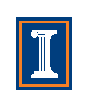
\includegraphics[height=1.5cm]{../images/imark_bold.eps}}

\begin{document}

\maketitle

\begin{frame}{Table of contents}
  \setbeamertemplate{section in toc}[sections numbered]
  \tableofcontents[hideallsubsections]
\end{frame}

\section{Background Information}

{%
\setbeamertemplate{frame footer}{Seeger, R.; Pople, J. A. J. Chem. Phys. 1977, 66 (7), 3045.
}
\begin{frame}[fragile]{Levels of Hartree-Fock Theory}
	\begin{center}
		\begin{tabular}{ | c | c | c | c |}
			\hline
			 \textbf{Method} & \textbf{Spinorbital} & \textbf{DoF} & \textbf{Eigenfunction of}\\
			\hline

			Restricted \rule{0pt}{7ex} &
			\begin{tabular}{c@{}c@{}}
				$\chi_j^\alpha(\vec{r},\sigma) =
				\sum\limits_{i=1}^{N} c_{ij}\phi_i\left(\vec{r \,}\right)\alpha(\sigma)$
				\\ \rule{0pt}{4ex}
				$\chi_j^\beta(\vec{r},\sigma) =
				\sum\limits_{i=1}^{N} c_{ij}\phi_i\left(\vec{r \,}\right)\beta(\sigma)$
			\end{tabular}
			& N/2
			& $\hat{S}^2$, $\hat{S}_z$
			\\ [5ex] \hline

			Unrestricted \rule{0pt}{7ex} &
			\begin{tabular}{c@{}c@{}}
			$\chi_j^\alpha(\vec{r},\sigma) = \sum\limits_{i=1}^{N}
			c_{ij}^\alpha\phi_i(\vec{r \,}) \alpha(\sigma)$
			\\ \rule{0pt}{4ex}
			$\chi_j^\beta(\vec{r},\sigma) = \sum\limits_{i=1}^{N}
			c_{ij}^\beta\phi_i(\vec{r \,}) \beta(\sigma)$
			\end{tabular}
			& N & $\hat{S}_z$ \\ [5ex]
			\hline

			General \rule{0pt}{7ex}&
			\begin{tabular}{r@{}r@{}}
				$\chi_j(\vec{r},\sigma) = \sum\limits_{i=1}^{N} [
				c_{ij}^\alpha\phi_i\left(\vec{r \,}\right) \alpha(\sigma) $
				\\ \rule{0pt}{4ex}
				$+c_{ij}^\beta \phi_i(\vec{r \,}) \beta(\sigma)]  $
			\end{tabular}
			& 2N & Neither \\ [5ex]
			\hline
		\end{tabular}
	\end{center}
\end{frame}

{%+
\setbeamertemplate{frame footer}{}


\begin{frame}[fragile]{Restricted Minimization}
	\begin{itemize}
		\item<1-> Hartee-Fock SCF guarantees only stationary energy w.r.t. change in orbitals
		\item<1-> The solution may be a maximum, minimum or saddle point
		\begin{itemize}
			\item<2->[] \begin{alertblock}{Within the Constrained Space} \end{alertblock}
		\end{itemize}
	\end{itemize}
	\begin{center}
		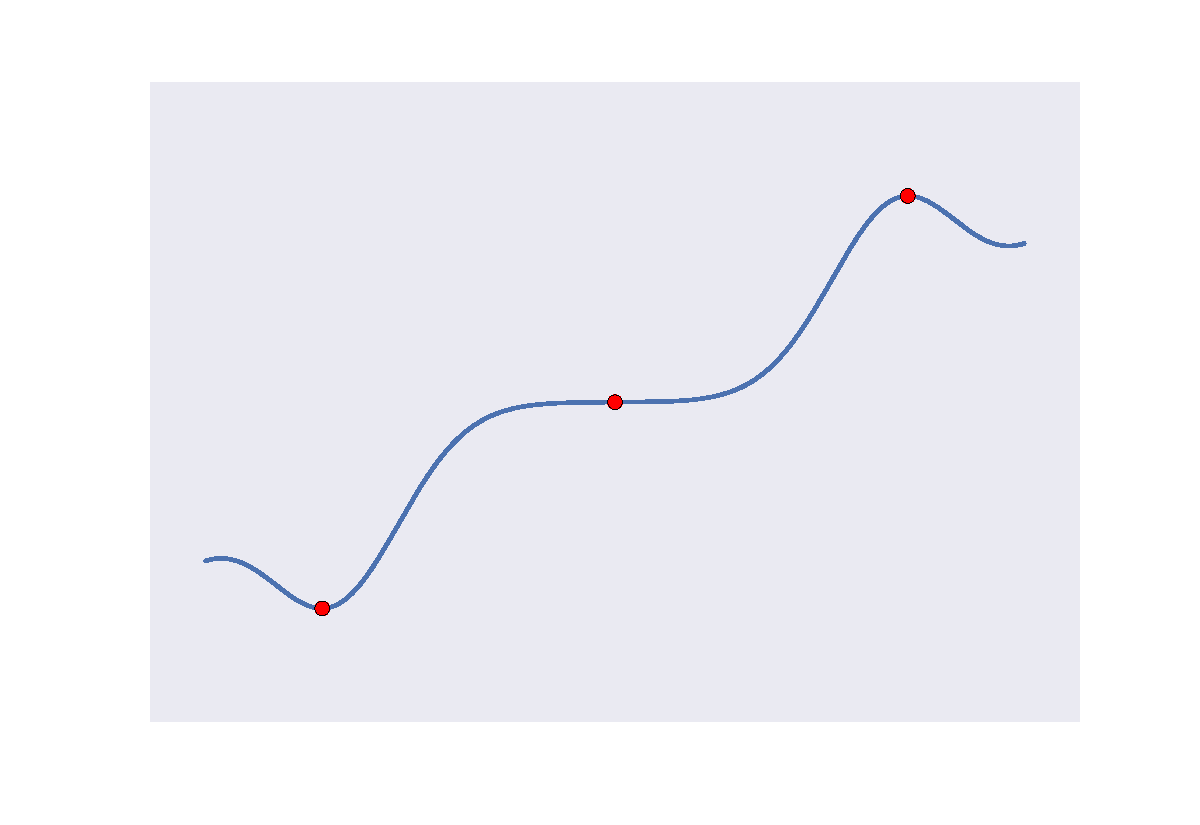
\includegraphics[width=0.5\textwidth, trim={3cm, 2cm, 3cm, 2cm}, clip]{../images/1d_extrema.pdf}
	\end{center}
\end{frame}

\begin{frame}{Restricted Minimization}
	\begin{columns}[c] % align columns
		\begin{column}{.48\textwidth}
			\begin{itemize}[<+->]
				\item {Restricted minima may correspond to minima in another dimension}
				\item {Restricted minima may correspond to maxima in another dimension}
				\item {Restricted minima may be nonstationary}
			\end{itemize}
		\end{column}
		\hfill
		\begin{column}{0.48\textwidth}
		    \begin{overprint}
			    \onslide<1>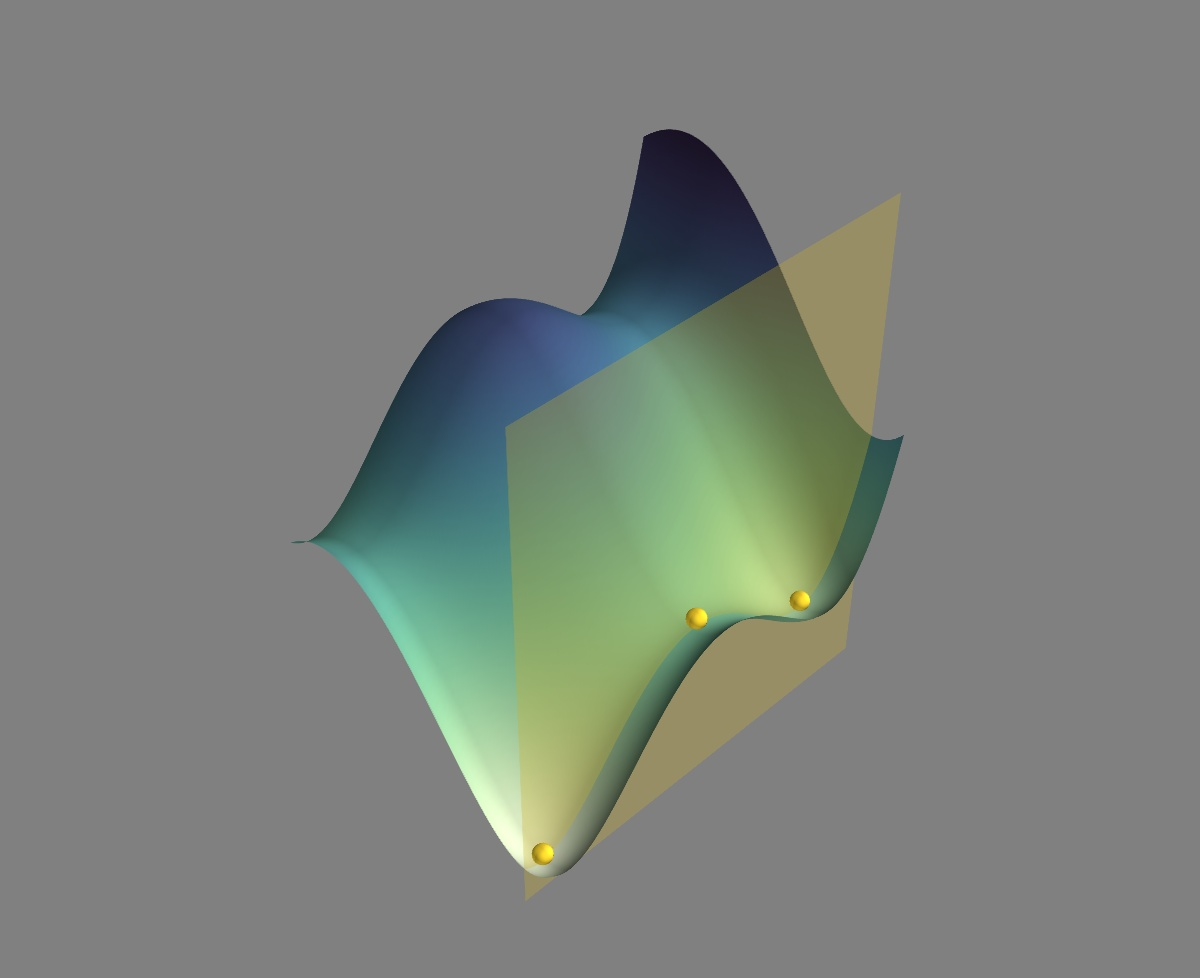
\includegraphics[width=0.9\linewidth, trim={7cm, 2cm, 7cm, 3cm}, clip]{../images/const_opt_globalmin.jpeg}
				\onslide<2>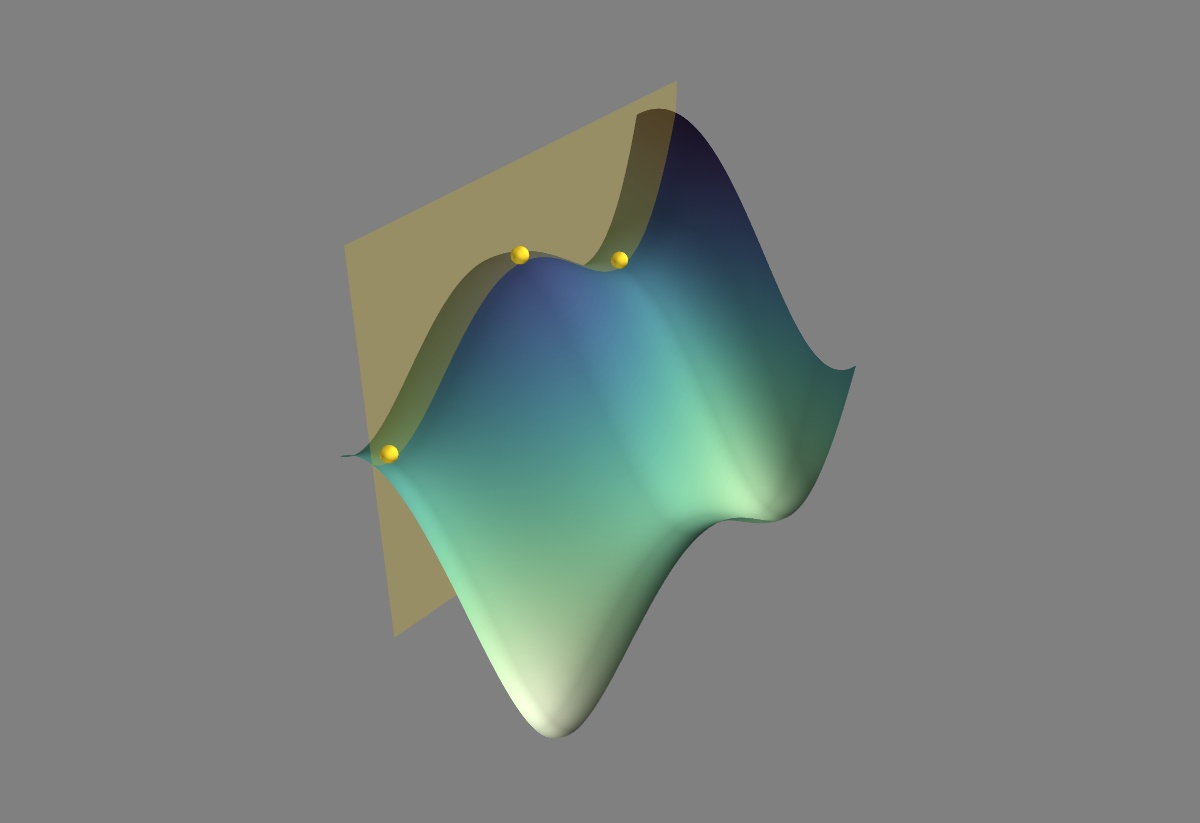
\includegraphics[width=0.9\linewidth, trim={7cm, 1cm, 7cm, 1cm}, clip]{../images/const_opt_saddle.jpeg}
				\onslide<3>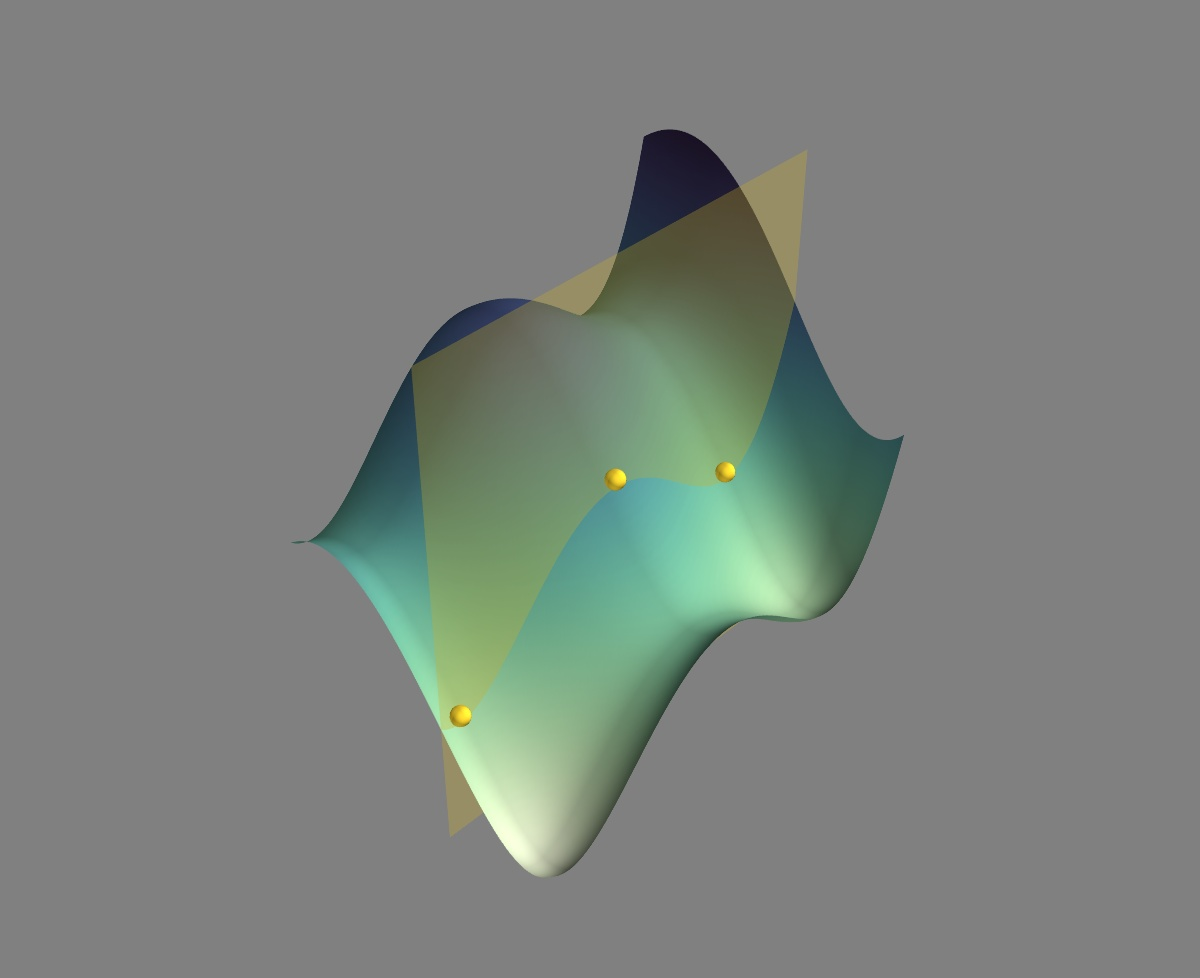
\includegraphics[width=0.9\linewidth, trim={7cm, 2cm, 7cm, 3cm}, clip]{../images/const_opt_nonstationary.jpeg}
			\end{overprint}
		\end{column}
	\end{columns}
\end{frame}


\section{Hartree-Fock Stability}

{%
	\setbeamertemplate{frame footer}{Thouless, D. J. The Quantum Mechanics of Many-Body Systems, 2nd ed.; Dover: 1972. (p. 114)}
\begin{frame}{Hartree-Fock Stability}
	\begin{itemize}[<+->]
		\item Solving the HF equations guarantees only that the energy is \alert{stationary}. The first order variation is therefore 0.
		\item We need to know if this is indeed a minimum.
		\item We can determine this if we inspect the \alert{second order variation} in the energy.
		\item Thouless$^1$ showed a physically motivated derivation using Time-Dependent Hartree-Fock theory (TDHF).
	\end{itemize}
\end{frame}

{%
	\setbeamertemplate{frame footer}{Thouless, D. J. The Quantum Mechanics of Many-Body Systems, 2nd ed.; Dover: 1972. (p. 114)}
\begin{frame}{Hartree-Fock Stability Conditions}
	\begin{itemize}[<+->]
		\item[]{The TDHF solution is given by the Liouville Von-Neumann Equation of Motion,
			\begin{eqnarray}
				i\hbar\frac{\partial \rho}{\partial t} = \left[ T+U, \rho \right],
			\end{eqnarray}
		}
		\item[]{Where U is the self-consistent potential,
			\begin{eqnarray}
				U_{pq} = \sum\limits_{p,q} \left(\rho_{pq,rs} - \braket{pr|sq} \right) \rho_{sr}.
			\end{eqnarray}
		}
		\item[]{Under the restrictions,
			\begin{eqnarray}
				\rho^2 = \rho \quad \textrm{and} \quad \rho^{\dagger} = \rho,
			\end{eqnarray}
		}
		\item[]{and to first order in $\rho_{ai}$, the elements of the density matrix are ,
			\begin{eqnarray}
				\rho_{ai} = C_{ai}, \quad \rho_{ia} = C_{ai}^*.
			\end{eqnarray}
		}
	\end{itemize}
\end{frame}

{%
	\setbeamertemplate{frame footer}{Thouless, D. J. The Quantum Mechanics of Many-Body Systems, 2nd ed.; Dover: 1972. (p. 114)}

\begin{frame}{Hartree-Fock Stability Conditions}
	\begin{itemize}[<+->]
		\item[]{The TDHF EoM becomes,
			\begin{eqnarray}
				i\hbar \frac{dC_{ai} \left(t\right) }{dt} &=& \left(\epsilon_a - \epsilon_i \right) \nonumber
					\\ &+& \sum\limits_{i}^{occ}  \sum\limits_{b}^{vir}
					  \left[\braket{aj||ib}C_{bj}   \left( t \right)
						  +\braket{ab||ij}C_{bj}^* \left( t \right) \right].
			\end{eqnarray}
		}
		\item[]{The solutions are complex exponentials,
			\begin{eqnarray}
				C_{ai} \left(t \right)  = \alpha X_{ai} e^{-i \omega t} + \alpha^* Y_{ai}^* e^{i \omega^* t},
			\end{eqnarray}
		}
		\item[]{whose amplitudes, $X_{ai}$ and $Y_{ai}$ satisfy,
			\begin{align}
				\left(\epsilon_a - \epsilon_i \right)X_{ai} + \sum\limits_{i}^{occ}  \sum\limits_{b}^{vir}
					\left[ \braket{aj||ib}X_{bj} + \braket{ab||ij}Y_{bj} \right] &= \hbar \omega X_{ai}
				\nonumber \\
				\left(\epsilon_a - \epsilon_i \right)Y_{ai} + \sum\limits_{i}^{occ}  \sum\limits_{b}^{vir}
					\left[ \braket{aj||ib}X_{bj} + \braket{ab||ij}Y_{bj} \right] &= -\hbar \omega Y_{ai}.
			\end{align}
		}
		\item[]{These are the equations of the Random Phase Approximation (RPA)}
	\end{itemize}
\end{frame}

{%
	\setbeamertemplate{frame footer}{Seeger, R.; Pople, J. A. J. Chem. Phys. 1977, 66 (7), 3045.}

\begin{frame}{Hartree-Fock Stability Conditions}
	\begin{itemize}[<+->]
		\item{The RPA frequencies represent electronic oscillations about the ground state}
		\item{Real frequencies are stable, imaginary frequencies are unstable}
		\item{The RPA frequencies are imaginary when the \alert{Orbital Hessian} (aka stability matrix, electronic Hessian) eigenvalues are \alert{negative}
			\begin{eqnarray}
				\begin{bmatrix}
					\bf{A}   & \bf{B}   \\
					\bf{B}^* & \bf{A}^* \\
				\end{bmatrix}
				\begin{bmatrix}  \bf{X} \\ \bf{Y}  \end{bmatrix}
				= \omega \begin{bmatrix}  \bf{X} \\ \bf{Y}  \end{bmatrix}
			\end{eqnarray}
		}
		\item{Where}
		\begin{eqnarray}
			A_{ia,jb} &=& \braket{{}_i^a|H-E_0|{}_j^b} = \left(\epsilon_a - \epsilon_i \right) \delta_{ij}\delta_{ab} + \braket{aj||ib}
			\nonumber \\
			B_{ia,jb} &=& \braket{{}_{ij}^{ab}|H-E_0|0} = \braket{ab||ij}.
		\end{eqnarray}
	\end{itemize}
\end{frame}

{%
	\setbeamertemplate{frame footer}{1) Seeger, R.; Pople, J. A. J. Chem. Phys. 1977, 66 (7), 3045.}
\begin{frame}{Hartree-Fock Stability Conditions}
	\begin{itemize}
		\item[]{The eigenvalue equation can be factorized depending on symmetry.} \\~\\
		\item[]{
			\resizebox{0.9\textwidth}{!}{%
			\begin{tabular}{r@{\qquad}cccccc}
				  \multirow{1}{*}{Solution Type} & \multicolumn{6}{c}{Space Type}  \\
				  \cmidrule{2-7}
				  & Real RHF & Complex RHF & Real UHF & Complex UHF & Real GHF & Complex GHF \\
				  \midrule
				  Real RHF    & ${}^1\mathbf{A}' + {}^1\mathbf{B}'$ & ${}^1\mathbf{A}' - {}^1\mathbf{B}'$ & ${}^3\mathbf{A}' + {}^3\mathbf{B}'$ & & & \\
				  Complex RHF & - & ${}^1\mathbf{H}'$ & - & \alert{${}^3\mathbf{H}'$} & - & \\
				  Real UHF    & - & - & $\mathbf{A}' + \mathbf{B}'$ & $\mathbf{A}' - \mathbf{B}'$ & $\mathbf{A}'' + \mathbf{B}''$ &  \\
				  Complex UHF & - & - & - &  $\mathbf{H}'$ & - & $\mathbf{H}'$ \\
				  Real GHF    & - & - & - & - & $\mathbf{A} - \mathbf{B}$ &  $\mathbf{A} - \mathbf{B}$  \\
				  Complex GHF & - & - & - & - & - & $\mathbf{H}$ \\
				  \bottomrule
			\end{tabular}}
		\item[] \tiny Table reproduced from Seeger \& Pople$^1$
		}
	\end{itemize}
\end{frame}

\section{Homogeneous Electron Gas}

{%
	\setbeamertemplate{frame footer}{Phillips, P. Advanced Solid State Physics, 2nd ed.; Cambridge University Press: Cambridge, 2012.}

\begin{frame}{Brief Overview}
	\begin{itemize}
		\item{Homogeneous Electron Gas (HEG) model, also known as Uniform Electron Gas or Jellium Model.}
		\item{Electrons in a box with "smeared" nuclei $\rightarrow$ uniform positive background charge}
		\item{The total charge is constrained to be neutral,}
			\begin{eqnarray}
				V_{bg}(\mathbf{r}) = \sum\limits_{i} \frac{-Ze^2}{|\mathbf{r}-\mathbf{R_i}|} \rightarrow -e^2 \int \frac{d\mathbf{r'}}{|\mathbf{r}-\mathbf{r'}|},
			\end{eqnarray}
		\item{and the background and coulomb terms cancel exactly,
			\begin{eqnarray}
				V_{ee} = e^2 \int \frac{d\mathbf{r'}}{|\mathbf{r}-\mathbf{r'}|}.
			\end{eqnarray}
		}
	\end{itemize}
\end{frame}

{%
	\setbeamertemplate{frame footer}{Giuliani, G.; Vignale, G. Quantum Theory of the Electron Liquid; 2005.}

\begin{frame}{Brief Overview}
	\begin{itemize}
		\item{The discretized solutions are given by,
		\begin{eqnarray}\label{eq:hf_orb_energy}
			\epsilon_{\vec{k}}=
				\frac{\hbar^2 k^2}{2m} - \sum\limits_{\vec{k}'}^{|\vec{k}'|< k_f}
				\braket{\vec{k}, \vec{k}' |\vec{k}', \vec{k}}
		\end{eqnarray}
		}
		\item{Where the two electron integral is given by
		\begin{align}
			\braket{\vec{k}, \vec{k}'|\vec{k}'',\vec{k}'''}\stackrel{\text{2D, 3D}}{=}&
				\begin{cases}
				\frac{\pi}{V}\frac{2^{D-1}}{|\vec{k}-\vec{k}''|^{D-1}}
				& \vec{k}''' = \vec{k}+\vec{k}'-\vec{k}'' \nonumber\\
				0
				& \text{else}
				\end{cases}
			\nonumber \\
			\braket{k, k'|k'',k'''}\stackrel{\text{1D}}{=}&
				\begin{cases}
				e^{|k-k''|^2a^2}\text{Ei}(-|k-k''|^2a^2)\text{ ;}
				& k''' = k+k'-k'' \\
				0\text{ ;}
				& \text{else}
				\end{cases}
		\end{align}
		}
	\end{itemize}
\end{frame}

\section{Notes on Iterative Subspace Eigenvalue Methods}
{%
\setbeamertemplate{frame footer}{1. Saad, Y. Numerical Methods for Large Eigenvalue Problems; SIAM, 2011.

 2. Davidson, E. R. J. Comput. Phys. 1975, 17 (1), 87–94.}
\begin{frame}{Subspace Methods in 1 Slide}
	\begin{itemize}
		\item{Sometimes the eigenvalue problem is too large to solve completely, and only a few eigenpairs are needed}
		\item{Subspace methods allow for finding some eigenpairs without full diagonalization}.
		\item{They need only a matrix-vector product (maybe diagonal elements too).}
		\item{A small subspace is constructed, then expanded slowly until the eigenpair residual norm,
			\begin{eqnarray}
				||\mathbf{Ax} - \lambda \mathbf{x}||,
			\end{eqnarray}
		is below some threshold.
		}
		\item{The \alert{Lanczos} and \alert{Arnoldi} methods are the most commonly used$^1$, while the \alert{Davidson}$^2$ method is likely more useful in a majority of chemical applications. }
	\end{itemize}
\end{frame}

{%
\setbeamertemplate{frame footer}{1. Saad, Y. Numerical Methods for Large Eigenvalue Problems; SIAM, 2011.

 2. Li, R.-C.; Zhang, L.-H. Convergence of Block Lanczos Method for Eigenvalue Clusters; 2013.}
\begin{frame}{Convergence Properties}
	\begin{itemize}[<+->]
		\item{The convergence of these subspace algorithms depends on:}
		\begin{itemize}
			\item{\alert{Number of eigenvalues} requested}
			\item{The \alert{block size} of the algorithm}
			\item{The \alert{density} of the eigenvalue spectrum}
			\item{The \alert{initial guess} eigenvectors}
			\item{The \alert{condition number} of the eigenvector matrix}
			\item{The \alert{preconditioner} (Davidson only)}
		\end{itemize}
		\item{They can \alert{converge to an incorrect answer} if:}
		\begin{itemize}
			\item{The block size is too small compared to degeneracy}
			\item{The approximate eigenvectors become non-orthogonal}
		\end{itemize}
		\item{My recommendation for guess eigenvectors is
		\begin{eqnarray}
			v_j^{(i)} = normalize\left(\frac{1}{|A_{ii} - A_{jj}| + 1} \right).
		\end{eqnarray}
		}
	\end{itemize}
\end{frame}


{%
\setbeamertemplate{frame footer}{Hern, V.; Tom, A.; Vidal, V. SLEPc Technical Reports, 2007.}
\begin{frame}{Orthogonalization}
	\begin{itemize}
		\item{The condition number, $\kappa$, is bound from below by
			\begin{eqnarray}
				\kappa \geq \frac{Max(A_{ii})}{Min(A_{jj})}
			\end{eqnarray}
		}
		\item{The Gram-Schmidt procedure has numerical issues,
			\begin{eqnarray}
				||\mathbf{I} - \mathbf{Q^TQ}|| \leq \frac{\alpha\kappa^2}{1-\beta\kappa^2}.
			\end{eqnarray}
		}
		\item{Modified Gram-Schmidt is better, but not perfect,
			\begin{eqnarray}
				||\mathbf{I} - \mathbf{Q^TQ}|| \leq \frac{\gamma\kappa}{1-\eta\kappa}
			\end{eqnarray}
		}
		\item{May need multiple orthogonalization steps}
	\end{itemize}

\end{frame}


{%
\setbeamertemplate{frame footer}{Overhauser, A. W. Phys. Rev. Lett. 1960, 4 (9), 462–465.}
\begin{frame}{Project Goal}
	\begin{itemize}[<+->]
		\item{Can we use the HF-Stability analysis to determine where the HEG is unstable?}
		\item{Will this predict the known tendency of crystallization at low density?}
		\item{It is known that the RHF-GHF instability persists at all densities for the HEG$^1$.}
		\item{Can we show this numerically, and discriminate between RHF-UHF and RHF-GHF instability?}
		\item{(Future) Can we combine this with to improve the efficacy of correlation theories (CC, MBPT)?}
	\end{itemize}
\end{frame}



\section{Results}

{%
\setbeamertemplate{frame footer}{}

\begin{frame}{First Brillouin Zone}
	\begin{columns}[c] % align columns
		\begin{column}{.4\textwidth}
			\begin{itemize}
				\item {Excite Ony in the X direction}
				\item {-X virtuals matter due to $\vec{k}' = \vec{k} + \vec{G}$}
			\end{itemize}
		\end{column}
		\hfill
		\begin{column}{0.6\textwidth}
		    \begin{overprint}
			    \onslide<1>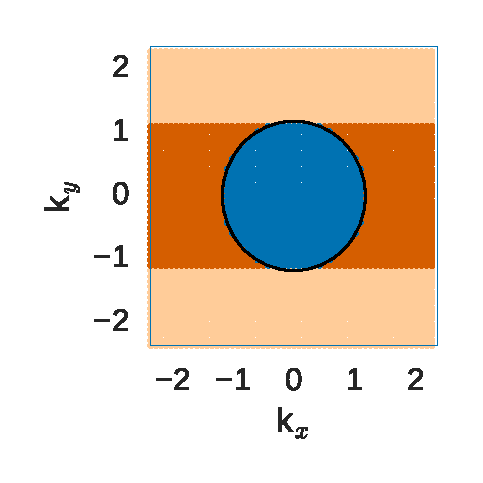
\includegraphics[width=\linewidth]{../images/1stBZ.eps}

			\end{overprint}
		\end{column}
	\end{columns}
\end{frame}

{%
\setbeamertemplate{frame footer}{}

\begin{frame}{Orbital Energies}
	\begin{columns}[c] % align columns
		\begin{column}{.4\textwidth}
			\begin{itemize}
				\item {Nk = 57 reproduces the orbital energies reasonably well}
				\item {Worst towards $\Gamma$, better for higher $|\vec{k}|$}
			\end{itemize}
		\end{column}
		\hfill
		\begin{column}{0.6\textwidth}
		    \begin{overprint}
			    \onslide<1>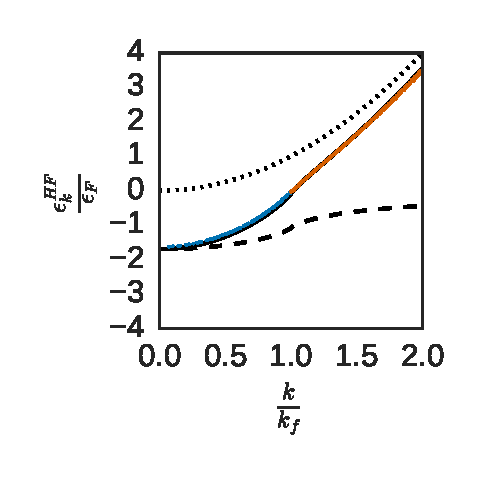
\includegraphics[width=\linewidth]{../images/energycompare.eps}

			\end{overprint}
		\end{column}
	\end{columns}
\end{frame}


{%
\setbeamertemplate{frame footer}{}

\begin{frame}{Matrix Diagonals}
	\begin{columns}[c] % align columns
		\begin{column}{.4\textwidth}
			\begin{itemize}
				\item {Spectrum is Dense}
			\end{itemize}
		\end{column}
		\hfill
		\begin{column}{0.6\textwidth}
		    \begin{overprint}
			    \onslide<1>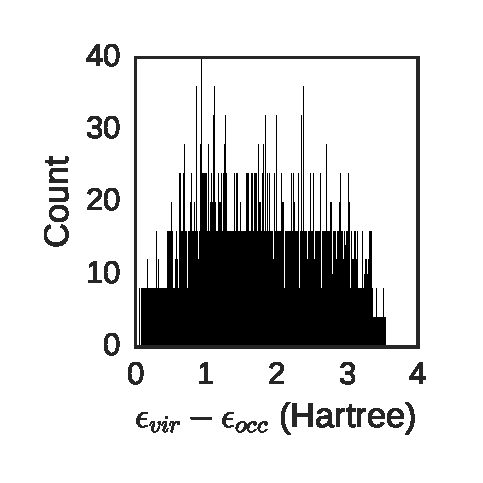
\includegraphics[width=\linewidth]{../images/exchist.eps}

			\end{overprint}
		\end{column}
	\end{columns}
\end{frame}



{%
\setbeamertemplate{frame footer}{}

\begin{frame}{Matrix Size Scaling}
	\begin{columns}[c] % align columns
		\begin{column}{.4\textwidth}
			\begin{itemize}
				\item {Scales as $2N_{exc}$}
				\item {$N_{occ}$ and $N_{vir}$ both scale with $N_{kpoints}^D$}
			\end{itemize}
		\end{column}
		\hfill
		\begin{column}{0.6\textwidth}
		    \begin{overprint}
			    \onslide<1>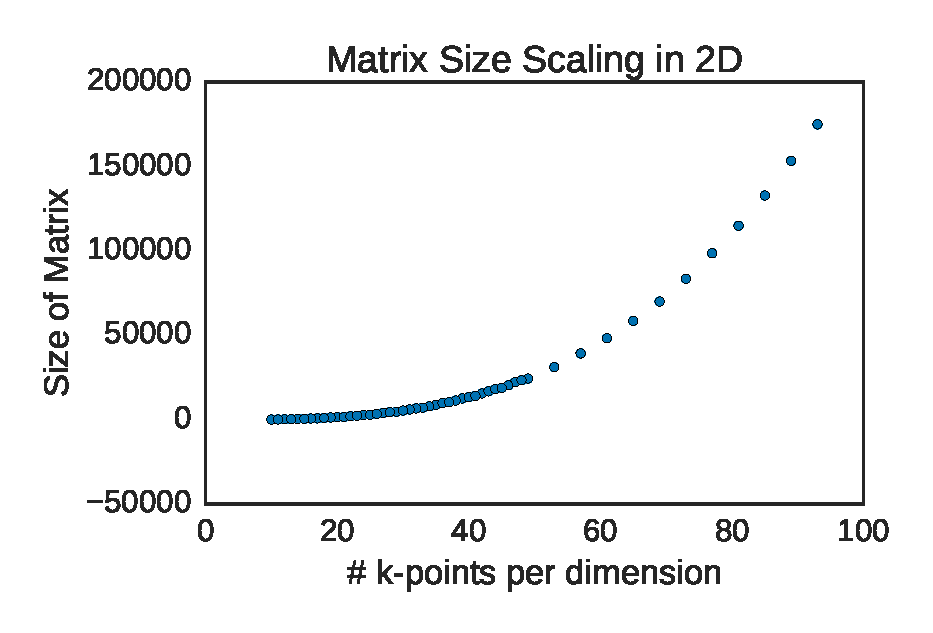
\includegraphics[width=\linewidth]{../images/matscale.eps}

			\end{overprint}
		\end{column}
	\end{columns}
\end{frame}


\begin{frame}{Matrix-Vector Scaling}
	\begin{columns}[c] % align columns
		\begin{column}{.4\textwidth}
			\begin{itemize}
				\item {Scales as $N_{exc} \times  N_{occ}$ due to momentum conservation}
			\end{itemize}
		\end{column}
		\hfill
		\begin{column}{0.6\textwidth}
		    \begin{overprint}
			    \onslide<1>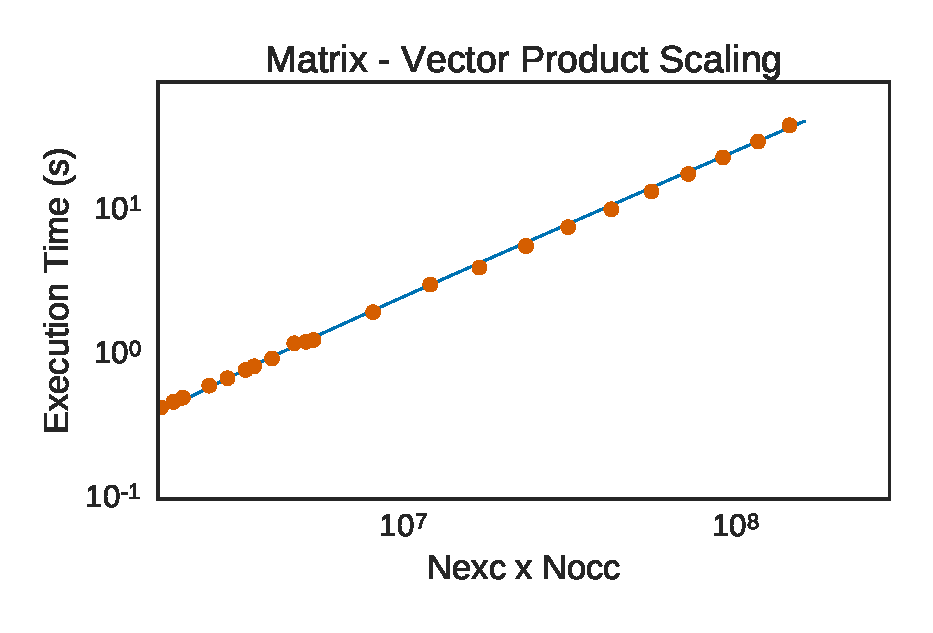
\includegraphics[width=\linewidth]{../images/mvscaling.eps}

			\end{overprint}
		\end{column}
	\end{columns}
\end{frame}

{%
\setbeamertemplate{frame footer}{1) http://mathworld.wolfram.com/StrassenFormulas.html}

\begin{frame}{Davidson Scaling}
	\begin{columns}[c] % align columns
		\begin{column}{.4\textwidth}
			\begin{itemize}
				\item {Davidson is Asymptotically quadratic.}
				\item {Full diagonalization is almost cubic.}
				\item {Matrix multiplication is order${}^1$ $log_2(7) \approx 2.807$}
			\end{itemize}
		\end{column}
		\hfill
		\begin{column}{0.6\textwidth}
		    \begin{overprint}
			    \onslide<1>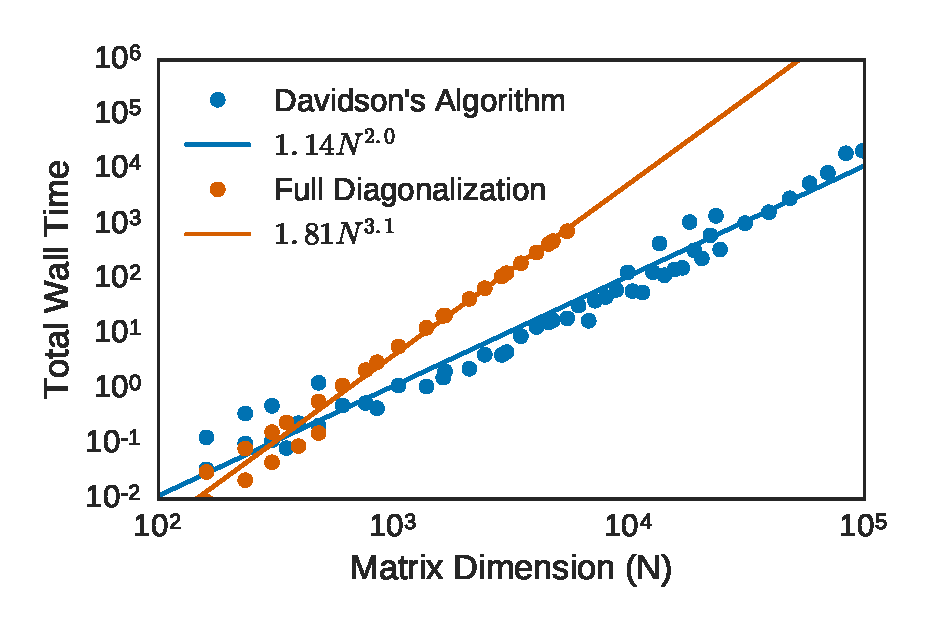
\includegraphics[width=\linewidth]{../images/dav_vs_exact_scaling.eps}

			\end{overprint}
		\end{column}
	\end{columns}
\end{frame}

\begin{frame}{Algorithm Wall time}
	\begin{columns}[c] % align columns
		\begin{column}{.4\textwidth}
			\begin{itemize}
				\item {Roughly quadratic wrt matrix dimension.}
				\item {Outliers correspond to high condition number}
			\end{itemize}
		\end{column}
		\hfill
		\begin{column}{0.6\textwidth}
		    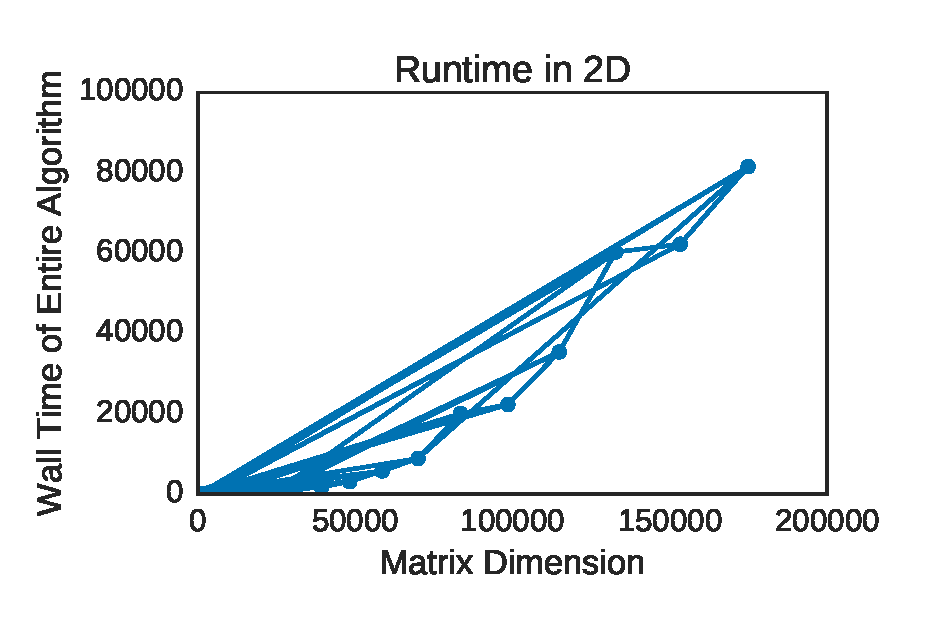
\includegraphics[width=\linewidth]{../images/overallruntime.eps}
		\end{column}
	\end{columns}
\end{frame}


\begin{frame}{Efficacy of Davidson's Algorithm}
	\begin{columns}[c] % align columns
		\begin{column}{.4\textwidth}
			\begin{itemize}
				\item {Reproduces Exact result to machine precision in all test cases.}
				\item {Odd spikes are due to approximating circle by squares}
			\end{itemize}
		\end{column}
		\hfill
		\begin{column}{0.6\textwidth}
		    \begin{overprint}
			    \onslide<1>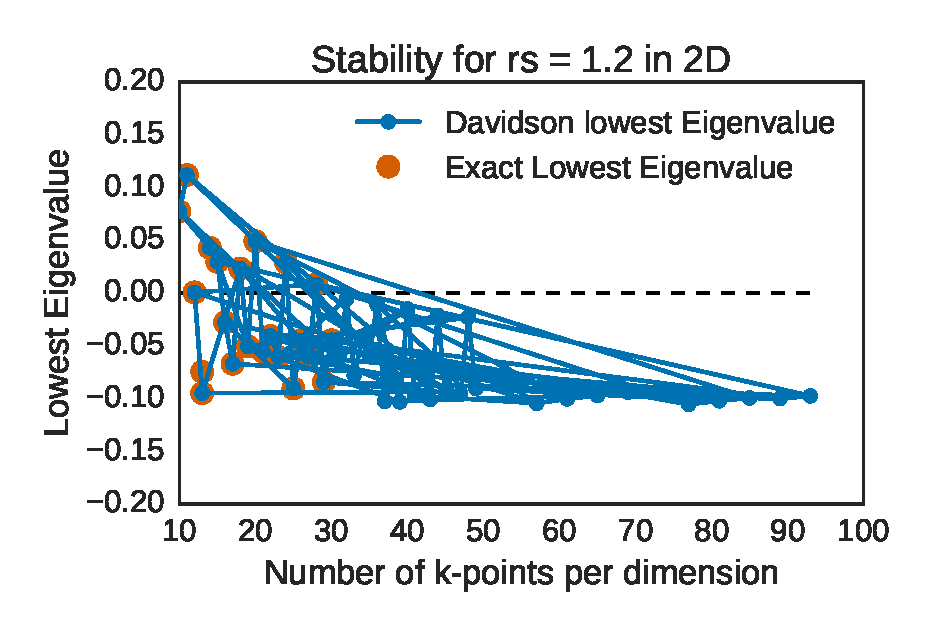
\includegraphics[width=\linewidth]{../images/dav_vs_exact.eps}

			\end{overprint}
		\end{column}
	\end{columns}
\end{frame}


{%
\setbeamertemplate{frame footer}{Bernu, B.; Delyon, F.; Holzmann, M.; Baguet, L. Phys. Rev. B 2011, 84 (11), 115115.}
\begin{frame}{Dependence on r${}_s$}
	Crossover from stable to unstable agrees with previous results.
	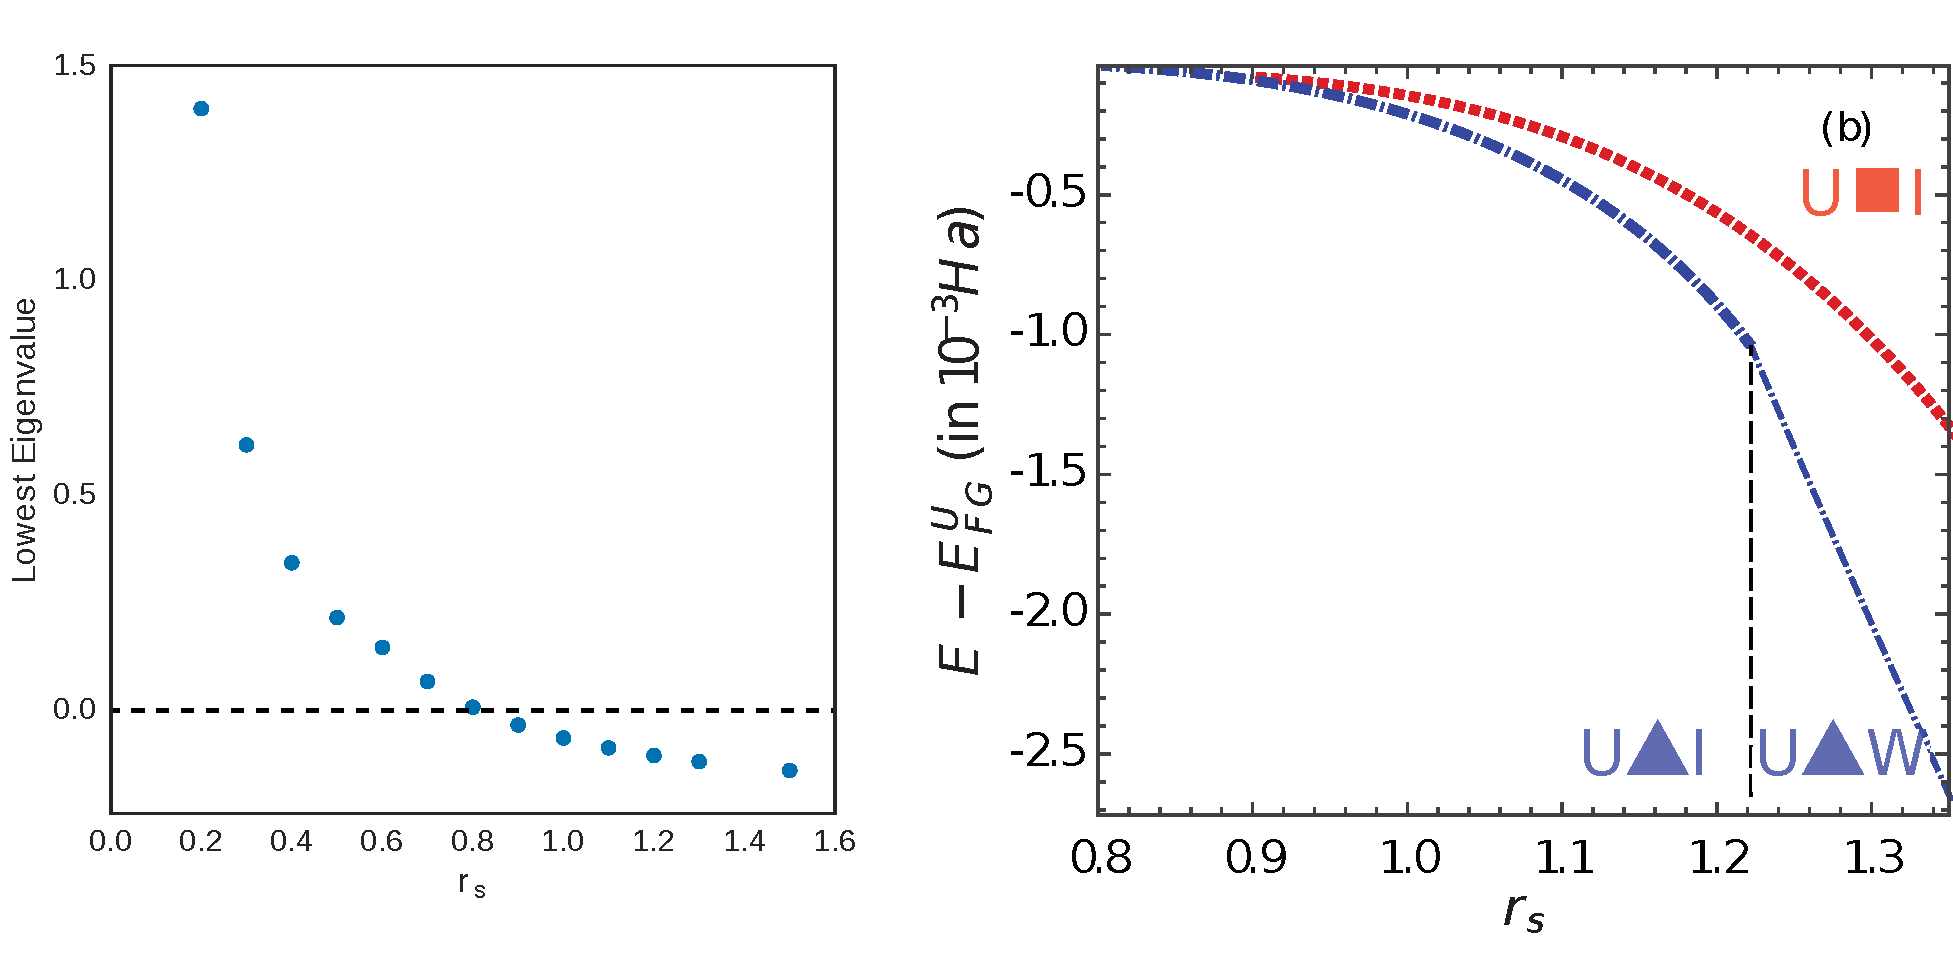
\includegraphics[width=.95\linewidth]{../images/MeVsBernu.pdf}
\end{frame}


\section{Concluding Remarks}

{%
\setbeamertemplate{frame footer}{}
\begin{frame}{Next Steps}
	\resizebox{\textwidth}{!}{%
	\begin{tabular}{l c c}
		Objective                 & Human Time   & Computer Time    \\
		\midrule
		Other instabilities in 2D & 30 mins & Week \\
		All 3D & $\frac{1}{2}$ Day&  $>$Weeks? Parallel?
	\end{tabular}}
\end{frame}
}

{%
\setbeamertemplate{frame footer}{}
\begin{frame}[standout]
  Questions?
\end{frame}

\appendix

%{%
%\setbeamertemplate{frame footer}{}
%\begin{frame}[fragile]{Backup slide}
%	Empty Backup
%\end{frame}
%
\end{document}
